% This is samplepaper.tex, a sample chapter demonstrating the
% LLNCS macro package for Springer Computer Science proceedings;
% Version 2.21 of 2022/01/12
%
\documentclass[runningheads]{llncs}
%
\usepackage[T1]{fontenc}
% T1 fonts will be used to generate the final print and online PDFs,
% so please use T1 fonts in your manuscript whenever possible.
% Other font encondings may result in incorrect characters.
%
\usepackage{graphicx}
% Used for displaying a sample figure. If possible, figure files should
% be included in EPS format.
%
% If you use the hyperref package, please uncomment the following two lines
% to display URLs in blue roman font according to Springer's eBook style:
%\usepackage{color}
%\renewcommand\UrlFont{\color{blue}\rmfamily}
%
\usepackage[ngerman]{babel}
\usepackage{wrapfig}
\begin{document}
%
\title{Gruppe 3: Catchphrase?}
%
%\titlerunning{Abbreviated paper title}
% If the paper title is too long for the running head, you can set
% an abbreviated paper title here
%
\author{...\inst{1}\and
...\inst{1}\and
...\inst{1}\and
...\inst{1}}
%
\authorrunning{F. Author et al.}
% First names are abbreviated in the running head.
% If there are more than two authors, 'et al.' is used.
%
\institute{FernUniversität in Hagen, Universitätsstraße 47, 58097 Hagen, Deutschland
\email{\{...\}@studium.fernuni-hagen.de}\\
\url{https://www.fernuni-hagen.de}}
%
\maketitle              % typeset the header of the contribution
%
%
\section{Einleitung}
Diese Arbeit wurde Rahmen des Fachpraktikums "`Multiagentenprogrammierung"' in einer Gruppenarbeit von vier Informatik-Studenten erstellt. Die Aufgabe umfasste die Bearbeitung des "`MASSim 2022: Agents Assemble III"' Szenarios \cite{EISMASSim}. Hierbei interagieren zwei oder mehr Teams auf einer 2-dimensionalen, aus Feldern bestehenden Karte. Jedes Team kontrolliert eine definierte Anzahl an Agenten, die verschiedene Aktionen ausführen können. Daneben existieren noch Hindernisse, Blöcke verschiedener Typen und sogenannte Dispenser, bei denen diese Blöcke erzeugt werden. Einige Felder der Karte sind als Zielzonen und Rollenzonen definiert. Ziel des Szenarios ist es, mithilfe der Agenten Blöcke zu sammeln, zu einer vorgegebenen Konfiguration zusammenzusetzen und in einer Zielzone abzugeben. Für jede erfolgreich bearbeitete Aufgabe gibt es Punkte. \\

Das Szenario läuft auf einem zentralen Server. Die Simulation ist rundenbasiert. Der Server sendet zu Beginn jeder Runde Informationen über die Umgebung an die Agenten. Diese verarbeiten die Informationen und senden die in der aktuellen Runde auszuführende Aktion an den Server. Dieser prüft die Eingaben der Agenten und aktualisiert den Zustand der Simulation. Die Aufgabe des Fachpraktikums besteht darin, das Agenten-Programm zu entwickeln. Dabei müssen die Agenten die Aufgaben möglichst effizient und kooperativ bearbeiten, um so viele Punkte wie möglich zu erzielen.

\section{Kommunikation und Kommunikationsmittel}
Die gruppeninterne Kommunikation erfolgte über den für das Fachpraktikum eingerichteten Discord-Server. Wir trafen uns jeden Mittwoch im Sprachchat der Gruppe, um anfangs die grundsätzliche Softwarearchitektur mittels UML-Diagrammen zu entwickeln und später über aktuelle Aufgaben und Probleme zu sprechen. Der Gruppen-Chat wurde darüber hinaus für kurzfristige Absprachen genutzt.\\

Die Quelltext-Verwaltung erfolgte über das Versionsverwaltungssystem Github, dessen Issue-Management wir ebenfalls verwendeten. Hier wurden alle Aufgaben zusammengetragen und jeweils ein Bearbeiter zugeordnet. Aus dem jeweiligen Issue wurde jeweils ein Feature Branch erstellt, in dem Bearbeitung der Aufgabe erfolgte. Abschließend wurden die Änderungen des Feature Branches mittels eines Pull Requests auf den Master Branch angewendet. Das Repositorium wurde so konfiguriert, dass ein Pull Request erst freigegeben wird, wenn er durch mindestens ein anderes Gruppenmitglied überprüft wurde. Dadurch sollte die Qualität des Quelltextes erhöht und das gemeinsame Verständnis des Quelltextes gefördert werden.


\section{Technische Rahmenbedingungen und Softwarebasisarchitektur}
Für die programmiertechnische Umsetzung entschieden wir uns für die Programmiersprache Java, da alle Gruppenmitglieder mindestens über grundlegende Kenntnisse dieser Programmiersprache verfügten. Außerdem ist Java eine stark typisierte Programmiersprache, wodurch einige Programmierfehler schon vor der Ausführung des Programms entdeckt werden können und so die Wahrscheinlichkeit von Laufzeitfehlern reduziert wird. Würde ein Laufzeitfehler während einer Simulation auftreten, dann müsste das Programm manuell neu gestartet werden. Während der Reaktionszeit bis zum Neustart läuft die Simulation (das Server-Programm) weiter. Für die während dieser Zeit laufenden Runden werden keine Aktionen gesendet, wodurch diese ungenutzt bleiben. Außerdem gehen alle bisher gesammelten Informationen (Objektzustände) verloren und müssen neu gesammelt werden.\\

Das objektorientierte Programmierparadigma, auf dem auch Java basiert, weist einige Gemeinsamkeiten mit dem Konzept der Agenten auf. Sowohl Objekte als auch Agenten besitzen einen gekapselten, inneren Zustand, führen Aktionen (Methoden) aus, um diesen Zustand zu verändern und kommunizieren mittels des Nachrichtenversands miteinander. Dennoch gibt es auch eine Reihe von Aspekten, die nicht standardmäßig im objektorientierten Programmierparadigma enthalten sind, aber trotzdem mithilfe objektorientierter Programmiersprachen implementiert werden können. Dazu zählt beispielsweise, dass eine Methode eines Objektes, solange sie öffentlich ist, jederzeit von anderen Objekten aufgerufen werden kann, während ein Agent selbst entscheidet, wann er eine Aktion ausführt. Ein weiterer Unterschied ist, dass Objekte in einem objektorientierten Programm standardmäßig nur einen gemeinsamen Ausführungsstrang aufweisen. Das Konzept der Agenten sieht hingegen einen eigenen Ausführungsstrang für jeden Agenten vor \cite{Weiss2000}.\\

Das in dieser Arbeit entwickelte Agentensystem basiert auf der BDI-Architektur. Diese Architektur ist eine Abstraktion des menschlichen Denkens bzw. Schlussfolgerns. Das heißt sie versucht zu beschreiben, wie Menschen sich für ihre nächste Handlung entscheiden, um dadurch übergeordnete Ziele zu erreichen. Die Komponenten der BDI-Architektur sind:
\begin{itemize}
\item{{\bf Beliefs:} Informationen, die der Agent über seine Umwelt besitzt}
\item{{\bf Desires:} Handlungsoptionen bzw. mögliche Ziele des Agenten}
\item{{\bf Intentions:} Ziele, für die sich der Agent entschieden hat und an deren Realisierung gerade gearbeitet wird}
\end{itemize}

Die Beliefs werden dabei durch eine Funktion auf Basis der Wahrnehmung der Umgebung und der aktuellen Beliefs aktualisiert. Die Desires werden aus den Beliefs und den aktuellen Intentions ermittelt. Die eigentliche Schlussfolgerung der nächsten Handlungen, also die Auswahl der Intentions, erfolgt durch eine Filter-Funktion, bei der die aktuellen Beliefs, Desires und Intentions einfließen. Der Vorteil dieser Architektur ist, dass eine funktionale Zerlegung des Agenten in die oben genannten Subsysteme vorgegeben ist. Die Komponenten erscheinen dabei intuitiv, da die BDI-Architektur auf dem menschlichen Denkmodell basiert \cite{Weiss2000}.\\

Auf der Grundlage der BDI-Architektur erarbeiteten wir anhand von Klassen-UML-Diagrammen konkrete Systemarchitekturen. Die UML-Diagramme stellen aufgrund der übersichtlichen, visuellen Darstellung des komplexen Systems eine gute Diskussionsgrundlage dar.

TODO Bdi, 2 Agentensysteme, UML, Java


\section{Gruppenbeitrag Heinz Stadler}
Nach einer ausführlichen Einarbeitung in die Thematik der Multiagentensysteme, erfolgte die Analyse der Ergebnisse des 15. Multi-Agent Programming Contest \cite{Ahlbrecht2021}. Diese ergab, dass neben der Entscheidungsfindung der Agenten, der Aufbau einer konsistenten und umfangreichen Wissensbasis (vgl. \cite[S. 29]{Ahlbrecht2021}) sowie die effiziente Problemfindung (vgl. \cite[S. 17]{Ahlbrecht2021}), eine wesentliche Schwierigkeit der Aufgabe bilden. \\
Als Folge dessen entschied sich der Autor mit dem Aufbau der Wissensverwaltung (siehe \ref{wissensverwaltung}) zu beginnen. Diese umfasst eine Datenstruktur zur Speicherung der von der Simulation übermittelten Informationen, sowie eine Lösung zum Aufbau einer globalen Karte des Simulationsgebiets. Nach Fertigstellung der Karte und deren funktionalen Verifikation, wurde parallel an der Konzeptionierung des Agentensystem V1 (siehe \ref{agentV1}) sowie der Implementierung einer intelligenten Wegführung (siehe \ref{wegfindung}) gearbeitet. Um die Ergebnisse der Wegführung und das Entscheidungsverhalten der Agenten effektiv verifizieren zu können, folgte die Erstellung eines graphischen Analysewerkzeugs (siehe \ref{verifikation}) das im weiten Entwicklungsverlauf stetig weiterentwickelt wurde und sich als sehr hilfreich bei der Fehlerfindung zeigte.
 
\subsection{Agent V1 - Architektur}\label{agentV1}
\begin{wrapfigure}{r}{0.56\linewidth}
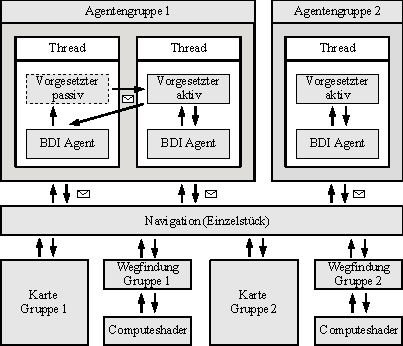
\includegraphics{./Referenzen/Architekturdiagramm.pdf}
\caption{Architekturdiagramm Agent V1}
\label{g3:architecture}
\end{wrapfigure}
Das Agentensystem V1 wurde vom Autor konzipiert, in der Gruppe abgestimmt und schließlich selbstständig implementiert. Es erweitert das BDI-Konzept \cite{Bratman1987} um zusätzliche Daten-, Berechnungs- und Entscheidungsebenen, die in Abbildung \ref{g3:architecture} illustriert sind. \\
Das System kombiniert den Aufbau eines BDI-Agenten (vgl. \cite[S. 58]{Weiss2000}) mit einer bidirektionalen vertikalen Schichtarchitektur \cite[S. 61-62]{Weiss2000}, auf die in Abschnitt
\ref{absichtsfindung} näher eingegangen wird.

Jeder Agent wurde mit einer Vorgesetzteninstanz, die eine zusätzliche Entscheidungsebene bildet, kombiniert und in einem Thread parallelisiert. Werden Agenten zu einer Gruppe zusammengeführt, bleibt eine Vorgesetzeninstanz aktiv. Die sonstigen Instanzen der Gruppe werden passiv und übernehmen im Weiteren nur noch die Weiterleitung von Nachrichten an die aktive Entität.

Die Kommunikation zwischen Instanzen in verschiedenen Threads erfolgt über Nachrichten, die in einer threadsicheren Warteschlange zwischengespeichert werden. Die Verständigung des Agenten mit seinem direkten Vorgesetzten wird mittels Methodenaufrufen realisiert.

Agentengruppen aktualisieren eine gemeinsame Karte mit im Simulationsverlauf erhaltenen Umgebungsinformationen. Diese und Module zur Wegführung werden von einem zentralem threadsicheren Navigationsmodul, das als Einzelstück ausgeführt wurde, verwaltet. 


\subsection{Wissensverwaltung}\label{wissensverwaltung}
Jeder Agent hat Zugriff auf eine individuelle Wissensbasis (Beliefs), die von der Simulation bereitgestellte Informationen auswertet und speichert. \\
Die enthaltenen Umgebungsdaten, beschränken sich auf das aktuelle Sichtfeld des Agenten. Es ist weder die Größe des Simulationsgebiets, noch die absolute Position des Agenten in diesem bekannt. 
Um aus den partiellen Umgebungsinformationen eine globale Sicht zu erhalten, werden diese an das Navigationsmodul weitergeleitet und in einer chronologisch fortgeschriebenen Karte zusammengeführt.

Beim Simulationsstart erhält jeder Agent, eine Karte mit festgelegter Initialgröße (Abb. \ref{Karte} Punkt 1), die beim Erkunden der Umgebung erweitert wird (Abb. \ref{Karte} Punkt 2). Treffen sich zwei Agenten aus unterschiedlichen Gruppen, wird dies vom Navigationsmodul erkannt und an die aktiven Vorgesetzten beiden Gruppen gemeldet. Stimmen beide Vorgesetzte einer Vereinigung zu, werden deren Karten überlagert und schließlich zusammengeführt (Abb. \ref{Karte} Punkt 3). Die entstandene Karte ermöglicht nun im weiteren Simulationsverlauf die aktuelle Position aller Agenten einer Gruppe untereinander zu bestimmen. Aus dieser Information kann nun durch jeweils zwei Agenten, die sich in entgegengesetzte Richtungen bewegen und sich durch das kontinuierliche Simulationsgebiet zwangsläufig wieder treffen, die Kartengröße ermittelt werden. Ist dies erfolgt, wird die Karte beschnitten, wobei die Informationen abgeschnittener Bereiche auf der gegenüberliegenden Seite eingefügt werden und somit nicht verloren gehen (Abb. \ref{Karte} Punkt 4).
\begin{figure}[h]
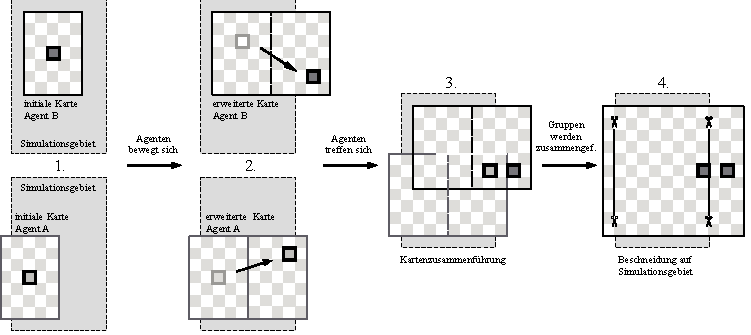
\includegraphics{./Referenzen/Kartenmerge.pdf}
\caption{Erweiterung und Zusammenführung einzelner Karten}
\label{Karte}
\end{figure}

\subsection{Wegfindung}\label{wegfindung}

\begin{wrapfigure}{r}{0.2\linewidth}
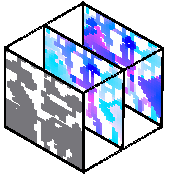
\includegraphics{./Referenzen/Pathfinding.pdf}
\caption{Datenstruktur Wegfindung}
\label{g3:architecture}
\end{wrapfigure}
Die 
Pathfinding, 2 Stufiges System

\subsection{Ziel- und Absichtsfindung}\label{absichtsfindung}
Desires, verticale Schichtarchitektur

\begin{wrapfigure}{r}{0.56\linewidth}
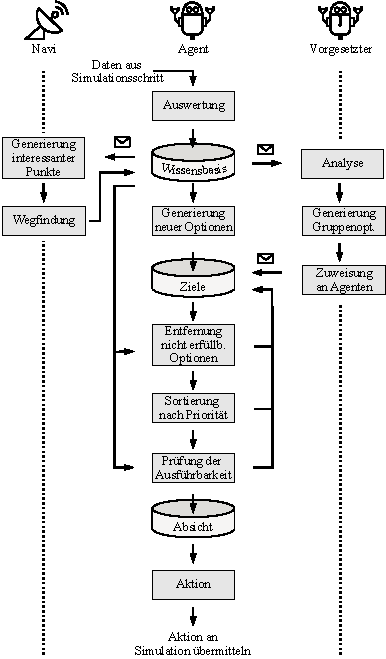
\includegraphics{./Referenzen/Entscheidungsfindung.pdf}
\caption{Architekturdiagramm Agent V1}
\label{g3:architecture}
\end{wrapfigure}

\subsection{Verifikation und Problemfindung}\label{verifikation}
Tests / Debugger

\subsection{Rekapitulation}
Zahlen, sonstiges Server Bug, Turnier gehalten, Github erstellt

\subsection{...}

\section{Gruppenbeitrag Melinda Betz}

\section{Gruppenbeitrag Phil Heger}
\subsection{Logging}
\subsection{Strategien zum Stören gegnerischer Agenten}
\subsubsection{Dispenser blockieren}
\subsubsection{Goal Zone verteidigen}

\section{Gruppenbeitrag Björn Wladasch}

\section{Turniere}
\subsubsection{Turnier 2}
\subsubsection{Turnier 3}
\subsubsection{Turnier 4}
\subsubsection{Turnier 5}
\subsubsection{Turnier 6}

\section{Rekapitulation und Ausblick}
Vor- und Nachteile der Entscheidung von zwei Architekturen
Was sollte noch verbessert werden
Wie sind wir zufrieden


%
% ---- Bibliography ----
%
% BibTeX users should specify bibliography style 'splncs04'.
% References will then be sorted and formatted in the correct style.
%
% \bibliographystyle{splncs04}
% \bibliography{mybibliography}
%
\begin{thebibliography}{8}
	\bibitem{Ahlbrecht2021}
	Ahlbrecht, T., Dix, J., Fiekas. N. und T. Krausburg: The Multi-Agent Programming Contest 2021, Springer, Heidelberg, 2021
	\bibitem{Hart1968}
	Hart, P. E., Nilsson, N. J. und Raphael, B.: A Formal Basis for the Heuristic Determination of Minimum Cost Paths, in IEEE Transactions on Systems Science and Cybernetics, 4. Auflage, Nummer 2, Seiten 100-107, Juli 1968
	\bibitem{Weiss2000}
	Weiss, G.: Multiagent Systems, 2. Auflage, The MIT Press, Cambridge, 2000
	\bibitem{EISMASSim}
	github.com/agentcontest/massim\_2022, agentcontest/massim\_2022, \\ https://github.com/agentcontest/massim\_2022/blob/main/docs/eismassim.md, EISMASSim Documentation, 21.08.2022
	\bibitem{Bratman1987}
	Bratman, M.: Intention, plans, and practical reason, Harvard University Press, Cambridge, 1987
\end{thebibliography}
\end{document}
